\chapter{Konzept}
\label{concept}
In den Abschnitten dieses Kapitels werden verschiedenen elementare Konzepte vorgestellt, welche im Prototyp zum Einsatz kommen. Nach einer Übersicht über das Grobkonzept werden Kernelemente und interaktive System erläutert um abschließend in \ref{sec:Spielfluss} das Zusammenspiel der einzelnen Systeme an einem kurzen fingierten Abenteuer aufzuzeigen.

\section{Spielkonzept}
\label{sec:Grobkonzept}

\begin{figure}[h]
	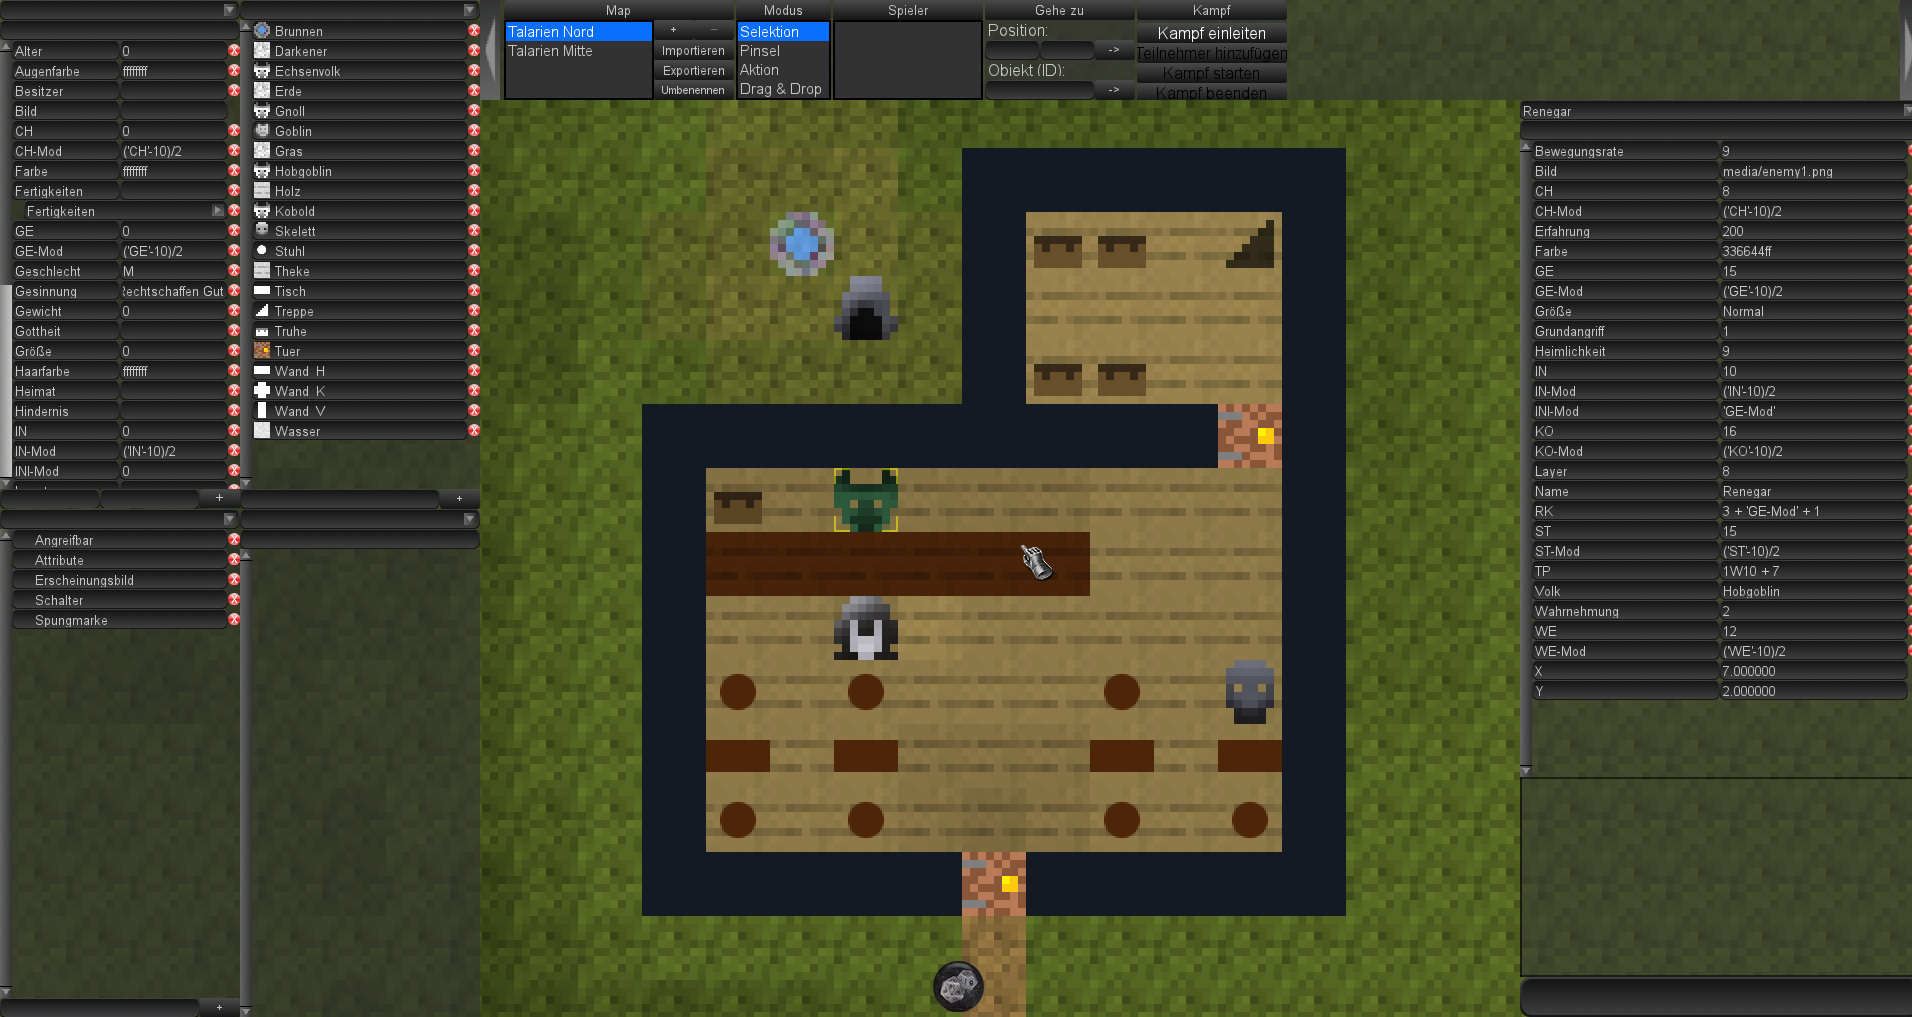
\includegraphics[width=\textwidth]{media/prototype}
	\caption{Beispielhafte Sicht des Spielleiters auf eine einfach Szene im Prototyp.}
\end{figure}

%\emph{Beschreibung des generellen Prototyps. Auf keinen Fall technisch.}
Der zur Beantwortung der Frage umgesetzte Prototyp benutzt eine einfache, zweidimensionale Darstellung um eine rudimentäre visuelle Repräsentation des Abenteuers bereitzustellen. Diese abstrakte Darstellung wurde bewusst gewählt um die Spieler dazu anzuregen weiterhin eine eigene Vorstellung der bespielten Welt zu pflegen. Mehrere Spieler~(Clients) verbinden sich mit einer Spielleiter-Instanz~(Server) über das Internet oder ein lokales Netzwerk. Der Prototyp implementiert verschiedene Komponenten welche das Durchführen einer PnP-Spielrunde mit dem analogen Original ähnlicher Stimmung und Spielfluss erlauben.



\subsection{Kernelemente}

%\begin{itemize}
%	\item Abstrakte Tile based world
%	\item Spielleiter kann Welt/jedes Objekt editieren
%	\item Spieler haben Echtzeit Rollenspiel + rundenbasierten Kampfmodus
%	\item Annahme: TeamSpeak oder ähnliche effective Kommunikation
%	\item Clienten (Spieler),  Server (GM)
%	\item Objectsystem, Rechtesystem
%\end{itemize}

\begin{figure}
	\centering
		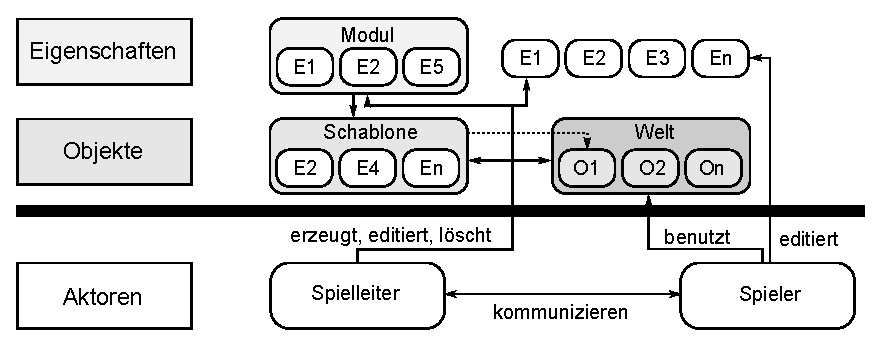
\includegraphics[width=1.00\textwidth]{media/konzept_schema.eps}
	\caption{Schematische Darstellung der komponentenbasierten Welt. Aktionen hängen nur von der Existenz und den Werten der Eigenschaften ab.}
	\label{fig:konzept_schema}
\end{figure}

Hauptkomponente des Prototyps ist ein frei definierbares Objektsystem. Zu jedem Zeitpunkt steht es dem Spielleiter frei Objekte und Werte derartig zu verändern, dass ein völlig anderes Vorgehen ermöglicht wird. Intern behandelt der Prototyp alle Elemente als gleichwertige Objekte. Diesen Objekten können verschiedene Eigenschaften zugeordnet werden, welche das Verhalten der Objekte definieren. Dieses System erlaubt es dem Spielleiter jedes Objekt in der Spielwelt zu editieren und bei Bedarf mit weiteren Daten anzureichern. Schlägt ein Spieler vor einen Gegenstand aus der Umgebung als Waffe zu nutzen, so kann der Spielleiter dem entsprechenden Objekt einen Schadenswert hinzufügen und diesen später in der Berechnung des Kampfwertes nutzen.\newline
Durch Module und Schablonen werden dem Spielleiter vorgefertigte Kombinationen von Eigenschaften und direkt verwendbare Objekte geliefert, welche er bei Bedarf schnell einsetzen kann. Mit dieser Option kann er das Verhalten der Spielwelt schnell ändern, was die Einwirkung bei laufendem Spiel ermöglicht.\newline
Ein internes Rechtesystem erlaubt es Spielern nur einen gewissen Teils dieser Eigenschaften zu sehen oder diese ändern zu können. Auf diese Weise kann er zwar z.B. seine Trefferpunkte selbst verwalten, aber keine beliebigen Gegenstände verändern.
Der Prototyp liefert in einer Anwendung eine Server- und eine Client-Ansicht aus. Der Spielleiter kann die Server-Ansicht nutzen um vor der Spielrunde das Abenteuer zu erstellen und leitet aus dieser Sicht heraus auch den Spielverlauf. Sobald der Server aktiviert wurde können sich die Spieler mit ihm verbinden und starten damit die Client-Ansicht. Um eine ähnlich flüssige Kommunikation wie bei analogen PnP-Runden zu ermöglichen wird davon ausgegangen, dass ein Echtzeitkommunikationsmedium wie z.B. Teamspeak\footnote{http://www.teamspeak.com/} oder Skype\footnote{http://www.skype.com/} genutzt wird. Zusätzlich bietet der Client noch einen einfachen Chat, über den Statusmeldungen, Spielernachrichten und verbal beschriebene Aktionen der Spielfiguren ausgegeben werden können.\newline
Die Interaktion der Spieler mit der Spielwelt geschieht in Echtzeit. Während eines Kampfes wechselt der Prototyp in das typische rundenbasierte Kampfsystem, welches auf dem D\&D-Regelsystem basiert. Dem Spielleiter stehen gleichzeitig alle Optionen offen, die Spielwelt im laufenden Spiel zu editieren.\newline
Durch die Kombination des offenen Objektsystems und der abstrakten Darstellung, welche schnell verändert oder durch eigene Grafiken erweitert werden kann, bietet der Prototyp damit ein Hilfsmittel um eigene, persönliche Abenteuer zu erstellen und in einer PnP-Runde zu durchspielen.

In \ref{fig:skillchain} wird ein Überblick über die wichtigsten Fertigkeiten eines Spielleiters gegeben. Es lässt sich gut erkennen das die meisten Fähigkeiten sich aus einer Nutzung der mitgelieferten Schablonen und Vorlagen entwickeln. Der Spielleiter beginnt die Schablonen nach eigenen Anforderungen an zu passen und kann schließlich mit dem nötigen Hintergrundwissen eigene Objekte umsetzen.

\begin{figure}[htbp]
	\centering
		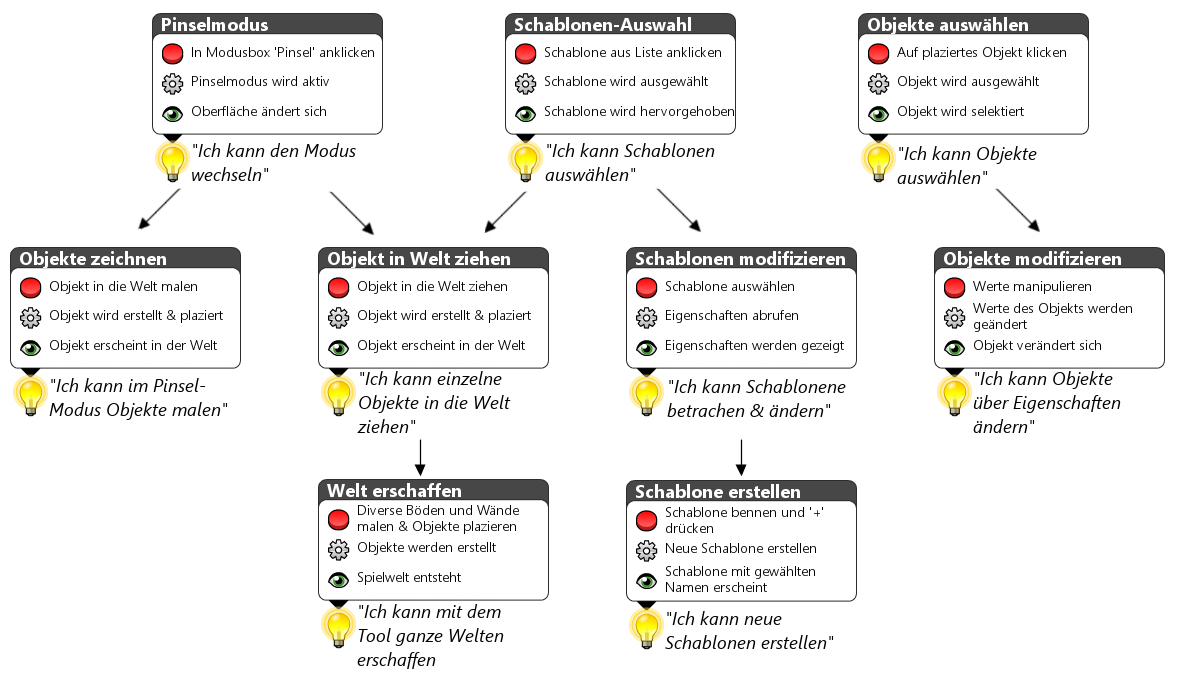
\includegraphics[width=1.00\textwidth]{media/skillchain.png}
	\caption{Auszug aus der schematischen Fähigkeitsentwicklung des Spielleiters}
	\label{fig:skillchain}
\end{figure}


\section{Interaktive Systeme}
\label{sec:InteraktiveSysteme}
Ein System veränderbarer Objekte erschafft zwar einen Baukasten, aber ein Spielfluss wird dadurch noch nicht realisiert. Das folgende Nachrichtensystem ist so allgemein gehalten, dass sich viele Aktionen direkt damit realisieren lassen. Das zusätzliche Kampfsystem setzt den häufig zentralen Teil des Kämpfens auf Basis des D\&D-Regelwerkes um.

\subsection{Kampfsystem}
\label{sec:Kampfsystem}
Ein großer Teil des D\&D-Regelwerkes befasst sich mit dem Ablauf von Kämpfen. Um den Aufwand überschaubar zu halten finden im Rahmen dieser Ausarbeitung nur die wichtigsten Regeln Beachtung. Diese Regeln werden im Folgenden kurz erklärt.~\cite{SRD35}

Der Kampf in D\&D läuft in Runden ab. Zu Beginn eines Kampfes führen alle Teilnehmer einen Initiativewurf durch, d.h. einen Wurf mit einem W20 auf den der u.a. von der Geschicklichkeit des Charakters abhängige Initiative-Modifikator addiert wird. Die Ergebnisse der Initiativewürfe bestimmen die Kampfreihenfolge, der Teilnehmer mit dem höchsten Initiativewert beginnt.\\
Die Runde eines Kampfteilnehmers besteht aus zwei großen Aktionsblöcken: \emph{Standardaktion} und \emph{Bewegungsaktion}. Mit der Standardaktion kann der Charakter jede Aktion ausführen, die im Regelbuch oder vom Spielleiter als solche deklariert wird. Dies sind z.B. ein einfacher Angriff oder das Wirken bestimmter Zauber. Die Bewegungsaktion erlaubt die Bewegung des Charakters über eine Distanz die nicht höher ist als seine Bewegungsrate. Dieser Wert hängt von der Rasse, Ausrüstung und anderen Faktoren des Charakters ab. Weiterhin kann die Bewegungsaktion durch eine bewegungsentsprechende Aktion ersetzt werden, z.B. das Laden einer schweren Armbrust oder das Aufstehen aus dem Liegen.\\
Aktionen, die eine komplette Runde in Anspruch nehmen (also Standard- und Bewegunsaktion verbrauchen) heißen \emph{Volle %SIC: im Regelbuch als Eigenname verwendet!
Aktion}. Eine häufig verwendete Aktion dieser Art ist der \emph{Volle Angriff}, bei dem mehrere Angriffsaktionen in einer Runde ausgeführt werden können.\\
Findet in der Runde keine tatsächliche Bewegung statt und verbietet keine der verwendeten Aktionen dies, so steht dem Teilnehmer ein 1,5m-Schritt zu.\\
Darüber hinaus gibt es weitere Aktionen, die keine oder sehr wenig Zeit in der Runde einnehmen und somit nach Ermessen des Spielleiters zusätzlich ausgeführt werden können. Diese Aktionen heißen \emph{Freie Aktion} oder \emph{Keine Aktion}.

Führt ein Kampfteilnehmer einen Angriff aus, so werden möglicherweise mehrere Würfe von ihm verlangt. Der erste Wurf heißt \emph{Angriffswurf}. Diese Probe gegen die Rüstungsklasse des Ziels bestimmt, ob der Angriff verfehlt, trifft oder sogar kritischen Schaden verursacht.\\
Bei einem erfolgreichen Angriff wird vom Angreifer ein \emph{Trefferwurf} ausgeführt. Dieser bestimmt wie viel Schaden das Ziel nimmt. Abhängig von der Waffe wird ein bestimmter Würfel verwendet. Nach Addition weiterer Werte wird der ermittelte Schaden von den Trefferpunkten (TP) des Ziels abgezogen. Sinken die TP des getroffenen Teilnehmers unter 0, so ist er ohnmächtig und kann nicht mehr agieren. Bei -10 Lebenspunkten ist der Charakter tot.

Für die genannten Regeln enthält der Prototyp ein Kampfsystem, welches den Ablauf steuert und die genannten Würfe verlangt. Über diese Regeln hinaus wurde bei der Konzeption des Prototyps darauf geachtet, dass auch andere Aktionen durch manuelles Eingreifen des Spielleiters möglich sind und nicht vom System unterbunden werden. Weiterhin wurde darauf geachtet, dass die Freiheit des Spielleiters nicht eingeschränkt wird. Sinken z.B. die TP eines Charakters durch Würfelglück eines Spielers unter -10 möchte der Spielleiter den getroffenen Charakter jedoch möglicherweise weiterkämpfen lassen, da ihm der Kampf zu einfach schien. Die Entscheidung den Charakter zu töten und zu entfernen wird also nicht automatisch vom System getroffen sondern liegt ultimativ beim Spielleiter.




\subsection{Nachrichtensystem}
\label{sec:Nachrichtensystem}
Während der Prototyp nicht auf ein Echtzeitkommunikationsmedium wie z.B. Teamspeak verzichten kann bietet er mit seinem Nachrichtensystem eine zusätzliche Mechanik an um den Informationsfluss im Spiel zu steuern. 
Über den Chat lassen sich Nachrichten und auch einfache \emph{Emotes} versenden. Dies soll im Spiel eine gewissen Form des Rollenspiels ermöglichen um zum Beispiel Gefühlsregungen des Charakters zum Ausdruck zu bringen, während ein anderer Teilnehmer gerade spricht. Verschiedene Ereignisse wie Würfelergebnisse oder das Auslösen eines Schalters werden ebenso im Chat ausgegeben wie Fehler in eingegebenen Formeln. Der Chat dient damit neben der Kommunikationsfunktion auch als Protokoll für das Abenteuer.\newline
Zusätzlich zum Chat können verschiedene Aktionen von Spielern oder vom Spielleiter gefordert werden, zum Beispiel das Auswürfeln der Initiative zum Kampfbeginn. Solche angeforderten Aktionen werden mit ihrem jeweiligen Symbol am unteren Bildschirmrand angezeigt und können minimiert, bzw. aufgeklappt werden.\newline
Eine wichtige Aktion dieser Art ist die \emph{Freitextaktion}, welche von einem Spieler auf ein beliebiges Objekt angewendet werden kann. Der Spielleiter erhält daraufhin eine solche Meldung mit dem Ausführenden und dem Ziel der Aktion, sowie dem vom Spieler eingegebenen Freitext. Der Spielleiter hat dann direkt in der Nachricht die Möglichkeit zu den betroffenen Objekte zu springen um die Situation zu analysieren und entsprechend zu entscheiden.


\section{Spielfluss}
\label{sec:Spielfluss}
In diesem Kapitel wird die Funktionsweise und das Zusammenspiel der verschiedenen vorgestellten Systeme anhand eines kurzen Abenteuers aus Sicht der Spieler und des Spielleiters erläutert.\newline
Der Spielleiter, im Folgenden auch \emph{SL} genannt, beginnt damit, ein Abenteuer zu konzipieren und vorzubereiten. In diesem Szenario sollen die Spieler in einer Taverne von dem Wirt beauftragt werden seltsamen Geräuschen aus dem Keller nachzugehen. Im Keller finden die Spieler einen Durchbruch in ein tieferes Gewölbe und müssen sich dort dem Kampf mit zwei Goblins stellen, um am Ende mit einer Schatztruhe belohnt zu werden.\newline
Im Anhang findet sich auf \ref{fig:storyflow_01}, \ref{fig:storyflow_02} und \ref{fig:storyflow_03} auch die Konzeption dieses Abenteuers, welches die Interaktionen von Spielleiter, Spieler 1 und Spieler 2 schematisch darstellt.

\subsection{Vorbereitung}
\label{sec:Vorbereitung}
Der SL beginnt seine Vorbereite mit dem Layout der Umgebung. Dafür greift er auf verschiedene generische Grafiken zu und nutzt die frei-definierbare Farbe um diverse Materialien wie z.B. Holz, Erde und Stein darzustellen. Auf dieser Grundlage erstellt er zwei verschiedene Karten, die Taverne und das Gewölbe, welches aus einem Eingangsbereich und einem größeren Raum für den Kampf und die Truhe besteht. Für die Gegner könnte der Spielleiter eine der vorbereiteten Schablonen nutzen, er entscheidet sich jedoch dafür einen eigenen Gegnertyp zu definieren. Dafür erstellt er ein neues Objekt und weist ihm eine Grafik zu. Danach fügt er das Modul \emph{'Angreifbar'} hinzu, welches die Eigenschaften \emph{'Trefferpunkte'} und \emph{'Rüstungsklasse'} enthält. Die Rüstungsklasse setzt der SL auf den festen Wert 12 und die Trefferpunkte auf 15.\newline
Der SL platziert nun zwei Instanzen der grade erstellen Schablone und eine Instanz der Truhen-Schablone in dem Verlies. Die Truhe besitzt die Eigenschaft \emph{'Inventar'}, die der Spielleiter nun mit einigen Münzen und einem Rüstungsobjekt befüllt. Zuletzt versiegelt der SL den Durchgang vom ersten in den zweiten Raum mit einigen bunten Balken, welche als Bücherregal fungieren werden. Einem Regal weißt der Spielleiter das 'Schalter' Modul zu, welches Spielern später die Möglichkeit der Interaktion gibt.\newline
Die Taverne füllt der Spielleitern mit einigen NPCs und Objekten, außerdem platziert er das Modul \emph{Sprungmarke} auf einer Tür im hinteren Bereich der Taverne und verbindet das Sprungziel mit dem ersten Raum der Gewölbekarte. Die Vorbereitung des Abenteuers ist hiermit abgeschlossen.

\subsection{Einführung in das Abenteuer}
\label{sec:EinführungInDasAbenteuer}


An der Spielrunde nehmen neben dem Spielleiter noch zwei Spieler (S1 und S2) teil. Nachdem beide Spieler mit einem an \emph{Pathfinder}\footnote{http://paizo.com/pathfinder}, eine Variante des D\&D-Regelwerkes, angelehnten Charakterbogen die Werte ihres Charakters definiert haben verbinden sie sich mit dem SL-Server. Der Prototyp synchronisiert nun die Spielwelt, Objektvorlagen und Medien des Spiels. Nachdem beide Spieler die Verbindung hergestellt haben platziert der Spielleiter sie in der Taverne.\newline
Die Spieler erkunden die Umgebung und bald entfaltet sich das Rollenspiel. 

\subsection{Rollenspiel}
\label{sec:Rollenspiel}

S1 fordert einen vom SL als besonders düster aussehend beschriebenen NPC zu einer Runde Armdrücken auf.\newline
Der Spielleiter würfelt verdeckt einen Wert für den NPC und fordert S1 auf ebenfalls eine Probe mit seinem Stärke-Modifikator auszuführen. Diese Eigenschaft ist an das Spielerobjekt angehängt und wird aus dem Wert des Stärke-Attributs errechnet. S1 merkt an, dass ihr Charakter eine hübsche, verschlagene Diebin ist und möchte gerne ebenfalls den Charisma-Modifikator mit einbringen. Der SL genehmigt dies und S1 würfelt endgültig mit \emph{1W20 + 'ST-Mod' + 'CH-Mod'}. S1 gewinnt diesen Wurf und als Preis erhält sie eine Runde Getränke aufs Haus.\newline
Nach einigen Getränken und Gesprächen mit den NPCs, welche der SL über Teamspeak durchführt, entscheiden sich die Spieler mit dem Abenteuer fortzuschreiten. 

\subsection{Das erste Rätsel}
\label{sec:DasErsteRätsel}

In einem Gespräch mit dem Wirt erfahren S1 und S2, dass es sonderbare Begebenheit im Keller der Taverne gibt. Der Spielleiter bewegt den Questgeber und gibt den Spielern so den Weg zur vorher definierten Sprungmarke frei.\newline
Voller Tatendrang und von den feinen Getränken ermutigt stürzen sich die Spieler in das Abenteuer. Nach der Interaktion mit der Sprungmarke werden beide Spieler automatisch auf der Gewölbekarte platziert. Der Spielleiter beschreibt die Umgebung kurz und lässt die Spieler dann die Umgebung selbst erkunden. Bald hat S2 herausgefunden, dass es die Möglichkeit gibt mit einem der Bücherregale zu interagieren. Der SL erhält die Benachrichtigung darüber über den Chat und entfernt das Bücherregal, während er eindrucksvoll beschreibt wie es sich unter Ächzen und Knarren im Boden versenkt.\newline


\subsection{Der Kampf}
\label{sec:DerKampf}
Die Spieler betreten den zweiten Raum und der Spielleiter fordert sie sofort auf eine Probe ihrer Schleichfähigkeit auszuführen. Das Würfelglück ist nun jedoch nicht bei den Spielern und daher startet ein Kampf mit den Goblins.\newline
Dafür selektiert der Spielleiter die Spieler und die Golbins und startet einen Kampf über seine GUI. S1 und S2 werden dadurch automatisch aufgefordert einen Initiative-Wurf abzulegen, der SL selbst würfelt diesen Wert für die Goblins aus. Es folgen einige Kampfrunden in denen Spieler und Goblins abwechselnd Angriffs- und Schadenswürfe sowie Bewegungen ausführen.\newline
Der Kampf endet siegreich für die Spieler. Sie können nun die Truhe im Raum untersuchen und sich an der reichen Beute bedienen. Der Spielleiter leitet die Spieler nun zurück in die Taverne und erzählt einen kurzen Abschluss des Abenteuers.


